\documentclass[12pt]{report}
\usepackage[utf8]{inputenc}
\usepackage{tabularx}
\usepackage{float}
\usepackage{graphicx}
\usepackage{hyperref}
\hypersetup{
    colorlinks,
    citecolor=black,
    filecolor=black,
    linkcolor=black,
    urlcolor=black
}
\usepackage{makeidx}
\makeindex

\title{Semi Anonymous image-based message board \\ 
        \large Software Project Management Document}
\author{Group No. 24\\Sahil Gangurde (2019IMT-034)\\Anish Jaiswal (2019IMT-017)\\Shashi Kumar (2019IMT-090)}
\date{ABV - Indian Institute of Information Technology, Gwalior}

\begin{document}

\maketitle

\newpage
\tableofcontents
\newpage

\chapter{Size Estimation}
It’s important to understand that project size estimation is the most fundamental parameter. If this is estimated accurately then all other parameters like effort, duration, cost, etc can be determined easily.
At present two techniques that are used to estimate project size are:
\begin{itemize}
    \item Lines of Code(LOC)
    \item Function Point
\end{itemize}

\section{Function Point Metric}
Function point metrics proposes that size of the software project is directly dependent on various functionalities it supports. More the features supported the more would be the size. This technique helps determine size of the project directly from the problem specification so is really helpful to project managers during project planning while determining size. For the purpose of our report, we will be using the Function Point metric to estimate the size.

\section{Unadjusted Function Point Estimation (UFP)}

\begin{itemize}
    \item Inputs
    \begin{enumerate}
        \item Personal Details for SignUp
        \item Username Password for Login
        \item Post Caption
        \item Board name
        \item Image path for upload
    \end{enumerate}
\end{itemize}

Number of inputs = 5

\begin{itemize}
    \item Outputs
    \begin{enumerate}
        \item Confirmation Message: User Successfully registered
        \item Confirmation Message: User Successfully Logged In
        \item Confirmation Message: Image Successfully Uploaded
        \item Confirmation Message: Post Successfully created
        \item Confirmation Message: Board Successfully created
        \item Error Message: Unsuccessful Sign Up
        \item Error Message: Unsuccessful Login
        \item Error Message: Unsupported Image format
        \item Error Message: Post not created
        \item Error Message: Board not created
        \item List of all posts created by user
        \item Information about User
    \end{enumerate}
\end{itemize}


Number of outputs = 12

\begin{itemize}
    \item Inquiries
    \begin{enumerate}
        \item View posts
        \item View boards
        \item View profile
    \end{enumerate}
\end{itemize}

Number of inquires = 3

\begin{itemize}
    \item Files
    \begin{enumerate}
        \item List of registered users
        \item List of posts
        \item List of images
    \end{enumerate}
\end{itemize}

Number of files = 3

\begin{itemize}
    \item Interfaces
    \begin{enumerate}
        \item User Module
    \end{enumerate}
\end{itemize}
Number of Interfaces = 1

To calculate UFP, we have,
\vspace{3pt}

\textbf{UFP} =  (Number of inputs)*4 + (Number of outputs)*5 + (Number of inquiries)*4 +(Number of files)*10 + (Number of interfaces)*10

\textbf{UFP} = 5*4 + 12*5 + 3*4 + 3*10 + 1*10 = \textbf{132}

\begin{itemize}
    \item Refine parameters
    \begin{enumerate}
        \item Inputs: 4 Simple + 1 Complex
        \item Outputs: 9 Simple + 3 Complex
        \item Inquiries: 3 Average
        \item Files: 3 Average
        \item Interfaces: 1 Complex
    \end{enumerate}
\end{itemize}

Refined UFP = 4*3 + 1*6 + 9*4 + 3*7 + 3*4 + 3*10 + 1*10 = 127

\begin{itemize}
    \item \textbf{Refine UFP based on overall complexity of the project}
    \begin{enumerate}
        \item Requirement for reliable backup and recovery = 5
        \item Requirement for data communication = 4
        \item Extent of distributed processing = 4
        \item Performance requirements = 4
        \item Expected operational environment = 4
        \item Extent of online data entries = 6
        \item Extent of multi-screen or multi-operation online data input = 4
        \item Extent of online updating of master files = 4
        \item Extent of complex inputs, outputs, online queries and files = 4
        \item Extent of complex data processing = 5
        \item Extent that currently developed code can be designed for reuse = 5
        \item Extent of conversion and installation included in the design = 1
        \item Extent of multiple installations in an organisation and variety of customer organisations = 4
        \item Extent of change and focus on ease of use = 5
    \end{enumerate}
    \item \textbf{Degree of influence} = 59
    \item \textbf{TCF} = 0.65 + 0.01*59 = 1.24
\end{itemize}

\vspace{1cm}

\textbf{Functional Point = UFP*TCF = 163.68}

\chapter{Effort and Time Estimation}

\section{COCOMO Model}

Boehm postulated that any software development project can be classified into one of the following three categories based on the development complexity—organic, semi detached, and embedded. This project belongs to the organic category. The basic COCOMO estimation model is given by expressions of the following forms:

\[ Effort = a_1 * (K_{LOC})^{a_2} PM \]

\[ T_{dev} = b_1 * (Effort)^{b_2} months \]

where, 
\begin{itemize}
    \item $K_{LOC}$ is the estimated size of the software product expressed in Kilo Lines Of Code
    \item $a_1$, $a_2$, $b_1$, $b_2$ are constants for each category of software product.
    \item $T_{dev}$ is the estimated time to develop the software, expressed in months.
    \item $Effort$ is the total effort required to develop the software product, expressed
in person-months (PMs).
\end{itemize}

\section{Estimation of development effort}
For our project we have estimated the size (in $K_{LOC}$) by analysing the already existing similar projects.
Estimated size = 3.9 $K_{LOC}$
Our application falls under the category of application softwares. So, the formulae for organic softwares will be used to calculate the effort and time of development.

\[ Effort = a_1 * (K_{LOC})^{a_2} PM \]
\[ = 2.4 * (K_{LOC})^{1.05} PM \]
\[ = 2.4 * (3.9)^{1.05} PM \]
\[ = 10.019 PM \]

\section{Estimation of development time}
\[ T_{dev} = b_1 * (Effort)^{b_2} months \]
\[ = 2.5 * (10.019)^{0.38} months \]
\[ = 6.001 months \]

\chapter{Project Schedule Breakdown}

\section{Activity Network}
An activity network shows different activities making up a project, their estimated durations, and their interdependencies. The activity diagram is shown in fig 3.1.

\begin{figure}[h]
\centering
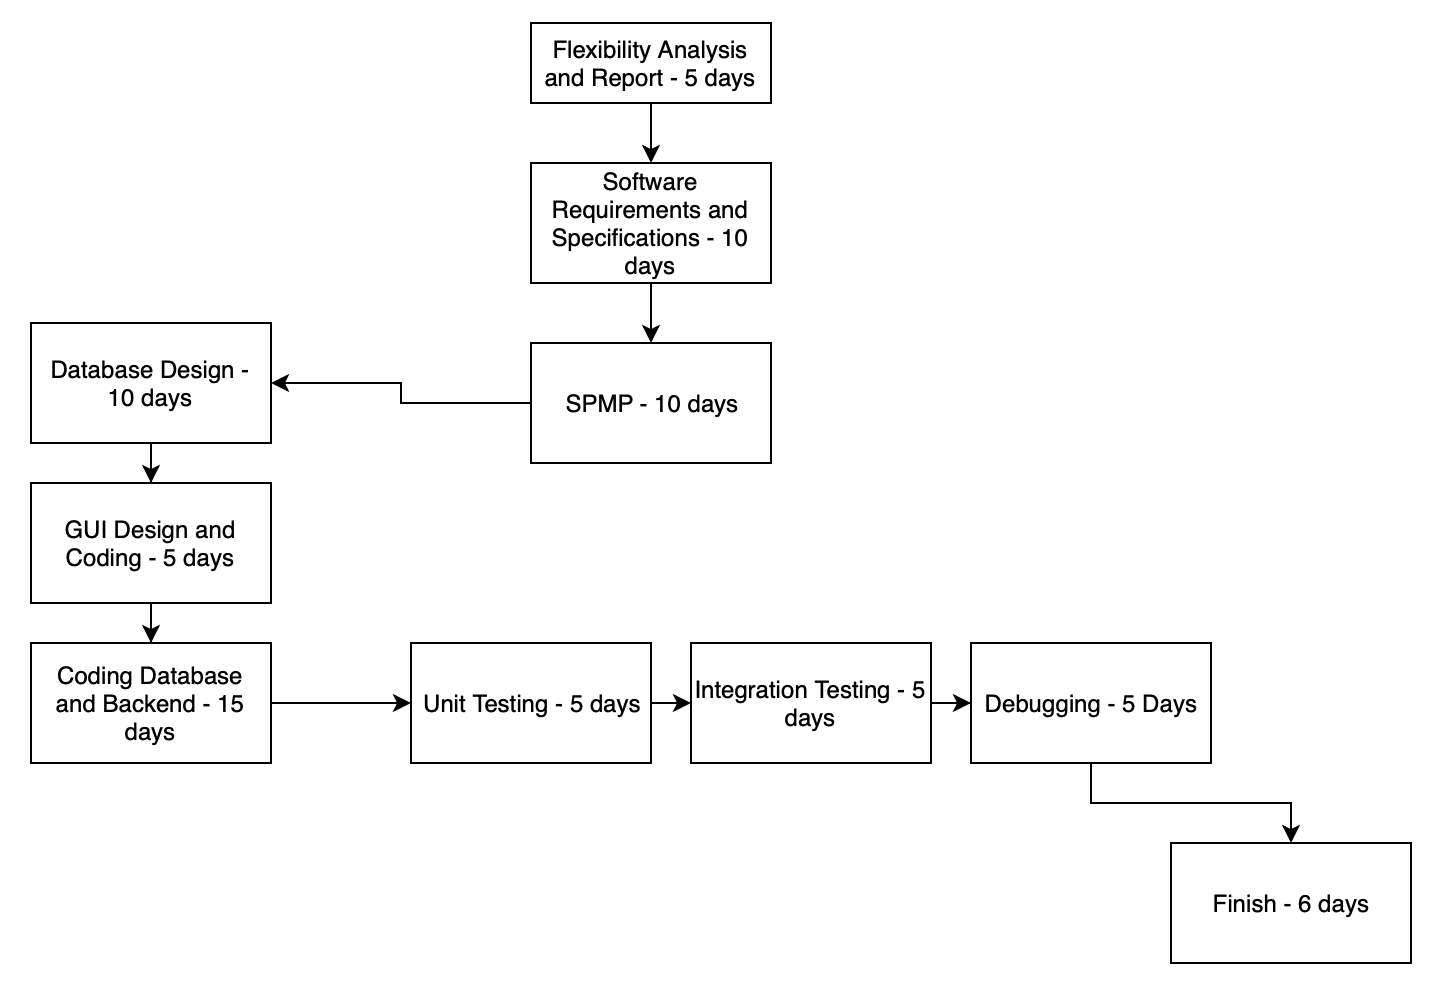
\includegraphics[width=15cm]{activitydiagram.png}
\caption{Activity Diagram}
\end{figure}

\section{PERT Chart}

Project evaluation and review technique (PERT) charts are a more sophisticated form of activity chart. PERT charts like activity networks consist of a network of boxes and arrows. The boxes represent activities and the arrows represent task dependencies. A PERT chart represents the statistical variations in the project estimates assuming these to be a normal distribution. PERT allows for some randomness in task completion times and therefore, provides the capability to determine the probability for achieving project milestones based on the probability of completing each task along the path to that milestone. See fig 3,2. Each task is annotated with three estimates:

\begin{itemize}
    \item Optimistic (O): The best possible case task completion time.
    \item Most likely estimate (M): Most likely task completion time.
    \item Worst case (W): The worst possible case task completion time.
\end{itemize}

\begin{figure}[h]
\centering
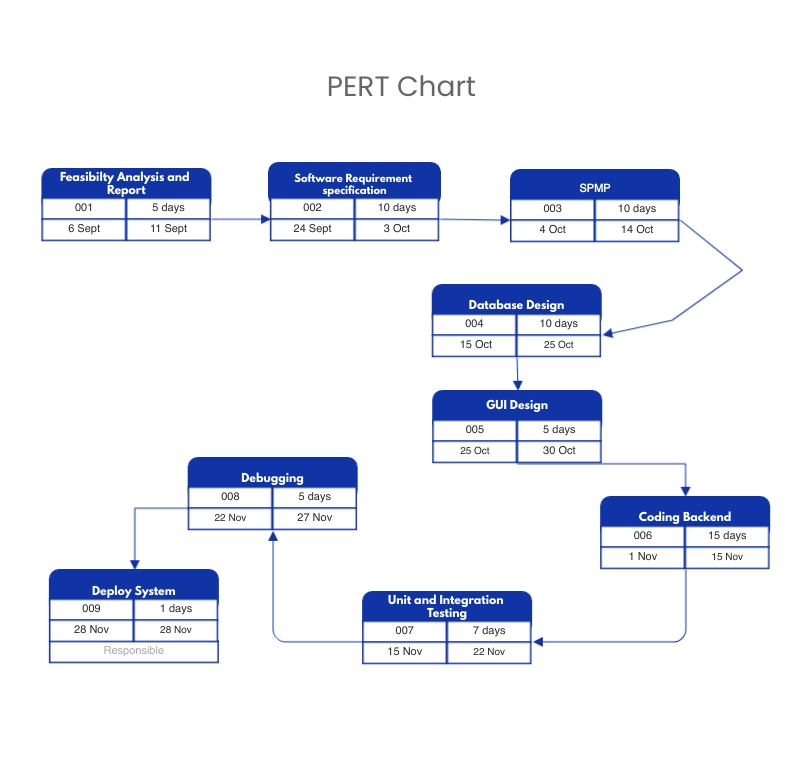
\includegraphics[width=15cm]{New-System-Implementation-PERT-Chart.jpg}
\caption{PERT Chart}
\end{figure}

\printindex





\end{document}
